\markboth{Battery Composition}{Battery Composition}
\section{Battery Composition}
The battery pack is modelled using a variation of the Composite design pattern with multiple composite classes\footnote{The basic Composite design pattern has one component interface, one composite class and one leaf class.}. This way, cells can be combined flexibly in various different topologies.

\subsection{Overview}
\label{sec:batteryCompositionOverview}
The \mcode{batteryInterface} is the abstract component that defines the interface for all objects in the composition. It is subclassed by all other battery elements. The \mcode{batteryCell} objects are the "leaves" and a composite can be one of the following classes:
\begin{itemize}
	\item \mcode{parallelElement}: A set of components in parallel.
	\item \mcode{seriesElementAE}: A set of components in series with active equalization.
	\item \mcode{seriesElementPE}: A set of components in series with passive equalization.
\end{itemize}
Each component can either be another composite object or a leaf.
\begin{figure}[b!]
	\captionsetup{type=figure}
	\centering
	\includegraphics[width=\textwidth]{topologies2.pdf}
	\caption[Visualization of the possible battery topology compositions]{Visualization of the possible battery topology compositions.}
	\label{fig:topologies2}
\end{figure}
Figure~\ref{fig:topologies2} provides a visual overview of the topologies that are possible using different compositions. Using this variation of the Composite design pattern, the components can be combined in any possible way at runtime. The most common battery topologies are strings of parallel elements (SP) and parallel strings of cells (PS)~\cite{cordoba-arenas_control-oriented_2015}. In Figure~\ref{fig:topologies2}, these would be the case if the composition's leaf nodes (cells) were all in the second layer (marked green). However, since every component can be either a cell or an array of other composite objects, more complicated topologies are made possible in this package. \\
\begin{figure}[t!]
	\captionsetup{type=figure}
	\centering
	\includegraphics[width=\textwidth]{composite_schema.pdf}
	\caption[Class diagram of the battery composition with communication flows and inheritance links]{Class diagram of the battery composition with communication flows and inheritance links.}
	\label{fig:composite_schema}
\end{figure}

\subsection{Method delegation}
\label{sec:method_delegation}
A pattern diagram of the classes used for the topology composition is depicted in Figure~\ref{fig:composite_schema}. Every composite element holds a reference to a component and delegates the methods called on it to said component. The delegated methods are wrapped with the rules of the respective topology in a similar fashion as is done with the Decorator design pattern. An example of the method delegation for a PS configuration - a \mcode{parallelElement} that holds a set of \mcode{seriesElement} objects, each in turn holding a set of \mcode{batteryCell} objects - is visualized in Figure~\ref{fig:method_delegation}. In this example, a current \mcode{I} and the simulation time step size is passed to the \mcode{parallelElement} via a \mcode{getVoltage()} method. The \mcode{parallelElement} determines which portion of \mcode{I} to send to each of it's components and delegates the method. Each \mcode{seriesElement} does the same and delegates the method to it's \mcode{batteryCell} objects. These return their voltages back to the \mcode{seriesElement} objects, which sum up the results received from their cells and pass the sum back to the \mcode{parallelElement}. Finally, the \mcode{parallelElement} calculates the mean of all the summed up voltages it received and passes the end-result back to the client.
\begin{figure}[t!]
	\captionsetup{type=figure}
	\centering
	\includegraphics[width=\textwidth]{method_delegation.pdf}
	\caption[Example of a method being delegated across a battery pack composition]{Example of a method being delegated across a battery pack composition.}
	\label{fig:method_delegation}
\end{figure}
The following operations are delegated by an object that implements the \mcode{batteryInterface}:
\begin{itemize}
	\item Determination of the new voltage after charging or discharging a with a certain current and time step size. This is delegated to each \mcode{batteryCell} object's \mcode{dischargeCurves} reference.
	\item Charging or discharging the battery.
	\item Determining the state of the battery if it were to be charged or discharged.
	\item Determining the maximum charging or discharging current.
	\item Calculating the pack's $SoH$.
	\item Getters and setters for the component's voltage and capacity properties.
	\item Getter for the component's internal impedance. 
\end{itemize}
With the number of subcomponents $n$, a component's voltage is determined as
\begin{equation} 
V\subi{component} = \left\lbrace
\begin{smallmatrix}
\frac{\sum_{i=1}^{n}V\subs{subcomponent}{i}}{n} & \text{for a parallel element}\\
& \\
\sum_{i=1}^{n}V\subs{subcomponent}{i} & \text{for a series element} \\
\end{smallmatrix}
\right.
\end{equation}
And a component's capacity is
\begin{equation}
C\subi{component} = \left\lbrace
\begin{smallmatrix}
\sum_{i=1}^{n}C\subs{subcomponent}{i} & \text{for a parallel element}\\
& \\
\min_{i=1}^{n}C\subs{subcomponent}{i} & \text{for a series element with passive equalization} \\
& \\
\frac{\sum_{i=1}^{n}C\subs{subcomponent}{i}}{n} & \text{for a series element with active equalization}\\
\end{smallmatrix}
\right.
\end{equation}
Since the $SoH$ is derived directly from the capacity (see Equation~\ref{eq:age_soh}), a component's $SoH$ can be determined in the same fashion.
\begin{equation}
SoH\subi{component} = \left\lbrace
\begin{smallmatrix}
\sum_{i=1}^{n}SoH\subs{subcomponent}{i} & \text{for a parallel element}\\
& \\
\min_{i=1}^{n}SoH\subs{subcomponent}{i} & \text{for a series element with passive equalization} \\
& \\
\frac{\sum_{i=1}^{n}SoH\subs{subcomponent}{i}}{n} & \text{for a series element with active equalization}\\
\end{smallmatrix}
\right.
\end{equation}
Due to the fact that the model is based on curve fits, the internal impedance $Z\subi{i}$ property is not used for modelling the charging behaviour directly. It does however, determine how the voltages and currents are distributed across the subcomponents when charging or discharging. The impedance proportionality factor $p\subi{z}$ of a subcomponent with index $j$ is the component's $Z\subi{i}$ divided by the sum of all subcomponents' $Z\subi{i}$.
\begin{equation}
p\subs{z}{j} = \frac{Z\subs{i}{j}}{\sum_{i=1}^{n}Z\subs{i}{i}}
\end{equation}
When charging, a series element with active equalization will distribute it's voltage equally across all of it's subcomponents to account for balancing, while a series element with passive equalization will distribute it's voltage according to $p\subs{z}{j}$. For a parallel element, the current is distributed in such a way that the subcomponent $j$ with the lowest $Z\subi{i}$ receives the highest current.
\begin{equation}
I\subs{subcomponent}{j} = \frac{\frac{1}{p\subs{z}{j}}}{\sum_{i=1}^{n}\frac{1}{p\subs{z}{i}}}
\cdot I\subi{component}
\end{equation}


\subsection{Battery Interface}
\label{sec:batteryInterface}
The battery interface is described in the following subsections. Every component implements the \mcode{batteryInterface}, so the methods described in this section can be called on \mcode{batteryCell} objects and on the composites.

\subsubsection{Battery object initialization}
To initialize a battery object at runtime, the nominal capacity $C\subi{n}$ in Ah and the nominal voltage $V\subi{n}$ in V must be passed to a \mcode{batteryCell} constructor. A composite can be initialized as an "empty" circuit element and the cell (or other composites) can be added to it via it's \mcode{addElements()} method\footnote{Here, "empty" is referred to in the sense of not holding any cells, not in the sense of an empty \matlab\ variable.}.

\begin{lstlisting}
% Initialize an "empty" parallel element
bat = parallelElement;
Cn = 3; % Nominal cell capacity in Ah
Vn = 3.2; % Nominal cell voltage in V
% Initialize 3 battery cells and add them to bat
for i = 1:3
	b = batteryCell(Cn, Vn);
	bat.addElements(b);
end
\end{lstlisting}
The \mcode{addElements()} method also accepts component arrays...
\begin{lstlisting}
for i = 1:3
	b(i) = batteryCell(Cn, Vn);
end
bat.addElements(b);
\end{lstlisting}
...and multiple inputs:
\begin{lstlisting}
b1 = batteryCell(Cn, Vn);
b2 = batteryCell(Cn, Vn);
b3 = batteryCell(Cn, Vn);
bat.addElements(b1, b2, b3);
\end{lstlisting}
To create a composition like the example in Figure~\ref{fig:method_delegation} (see also Figure~\ref{fig:topologies2}, right), the following syntax could be used:
\begin{lstlisting}
% Initialize "empty" parallel element
bat = parallelElement;
% Initialize 3 "empty" series elements each holding 3 cells
for i = 1:3
	se = seriesElementPE; % passive equalization
	for j = 1:3
		se.addElements(batteryCell(Cn, Vn))
	end
	% Add series elements to bat
	bat.addElements(se)
end
% Further initialization operations, e.g. bat.addcurves() here...
\end{lstlisting}

\subsubsection{Battery charging and discharging}
\label{sec:charge_discharge}
Battery charging \footnote{Discharging will also be referred to as charging (with a negative current) in this documentation.} is handled by the methods \mcode{powerRequest()} and \mcode{currentRequest()}. Both functions are called in a similar manner. The syntax is as follows:
\begin{lstlisting}
[P, V, I] = bat.powerRequest(P, dt);
[P, V, I] = powerRequest(bat, P, dt); % equivalent
[P, V, I] = bat.currentRequest(I, dt);
[P, V, I] = currentRequest(b, I, dt); % equivalent
\end{lstlisting}
Where \mcode{P} is the requested power $P$ in W, \mcode{I} is the requested current $I$ in A and \mcode{dt} is the simulation time step size $\Delta t\subi{s}$ in s. The methods return the actual power throughput in W, the battery's voltage $V$ at the end of the time step and the actual current throughput in A. The returned power and current is limited by the $SoC$ or the cells' maximum currents, among other factors.
\begin{figure}[b!]
	\captionsetup{type=figure}
	\centering
	\includegraphics[width=\textwidth]{powerRequest.pdf}
	\caption[Flow chart of the \mcode{powerRequest()} and \mcode{currentRequest()} methods]{Flow chart of the \mcode{powerRequest()} and \mcode{currentRequest()} methods.}
	\label{fig:powerRequest}
\end{figure}
Figure~\ref{fig:powerRequest} contains a flow chart of the charging process. The client sends a request to the battery. If the requested power is not equal to zero and the battery's $SoC$ is not already at it's upper or lower limit, a charge iteration is performed (the \mcode{iteratePower()} and \mcode{iterateCurrent()} methods are called, respectively) and the resulting power, current and voltage are returned to the client. A positive input to the charge iteration  indicates charging and a negative input specifies discharging. If the request is zero, signalling that the battery is in an idle state, a logical flag is set to true and the charge iteration is called with the battery's self-discharge $P\subi{sd}$. The logical flag is checked after every call to the charge iteration methods in order to return a power and current of zero to the client if it was set to true. If the $SoC$ is either at it's upper or lower limit, the battery simply returns it's voltage along with a power and current of zero.\\
\begin{figure}[t!]
	\captionsetup{type=figure}
	\centering
	\includegraphics[width=\textwidth]{iteratePower.pdf}
	\caption[Flow chart of the \mcode{iteratePower()} method]{Flow chart of the \mcode{iteratePower()} method.}
	\label{fig:iteratePower}
\end{figure}
A flow chart of the \mcode{iteratePower()} method is depicted in Figure~\ref{fig:iteratePower}. First, a current is estimated from the requested power and the battery's voltage. The current and the time step size are then delegated to the battery cells' \mcode{dischargeCurves} objects, in order to determine the resulting voltage. An approximation of the power is determined from the mean of the returned voltage and the battery's old voltage. This is repeated through recursion until the difference between the iterated power and the originally requested power meets a certain tolerance. If the resulting current is greater than the battery's maximum current $I\subi{max}$, the \mcode{iterateCurrent()} method is called using $I\subi{max}$ as an input. It's output current, the resulting power and voltage are returned. Otherwise, the $SoC$ is determined and compared the battery's upper and lower limit. If the $SoC$ is within the interval $[SoC\subi{min}, SoC\subi{max}]$, the power, current and voltage are returned. Otherwise, the requested power is adjusted according to the difference between the $SoC$ and the respective limit that was exceeded, thus starting the iteration again. \\
\begin{figure}[t!]
	\captionsetup{type=figure}
	\centering
	\includegraphics[width=\textwidth]{iterateCurrent.pdf}
	\caption[Flow chart of the \mcode{iterateCurrent()} method]{Flow chart of the \mcode{iterateCurrent()} method.}
	\label{fig:iterateCurrent}
\end{figure}
Figure~\ref{fig:iterateCurrent} depicts a flow chart of the \mcode{iterateCurrent()} function. Using this method is a lot faster than using the \mcode{iteratePower()} function, due to it's comparative simplicity. However, the current may need to be determined separately in some cases. Before the iteration, the current is limited to $I\subi{max}$. Finally, the another limitation is performed if the $SoC$ is not within the interval $[SoC\subi{min}, SoC\subi{max}]$. Normally, one or two iterations should suffice for returning the current and $SoC$. The voltage and power are not calculated and must be determined by calling the \mcode{getNewVoltage()} method if required\footnote{For example, this is done within the \mcode{currentRequest()} method, which does return the voltage and power.}.\\
\begin{figure}[t!]
	\captionsetup{type=figure}
	\centering
	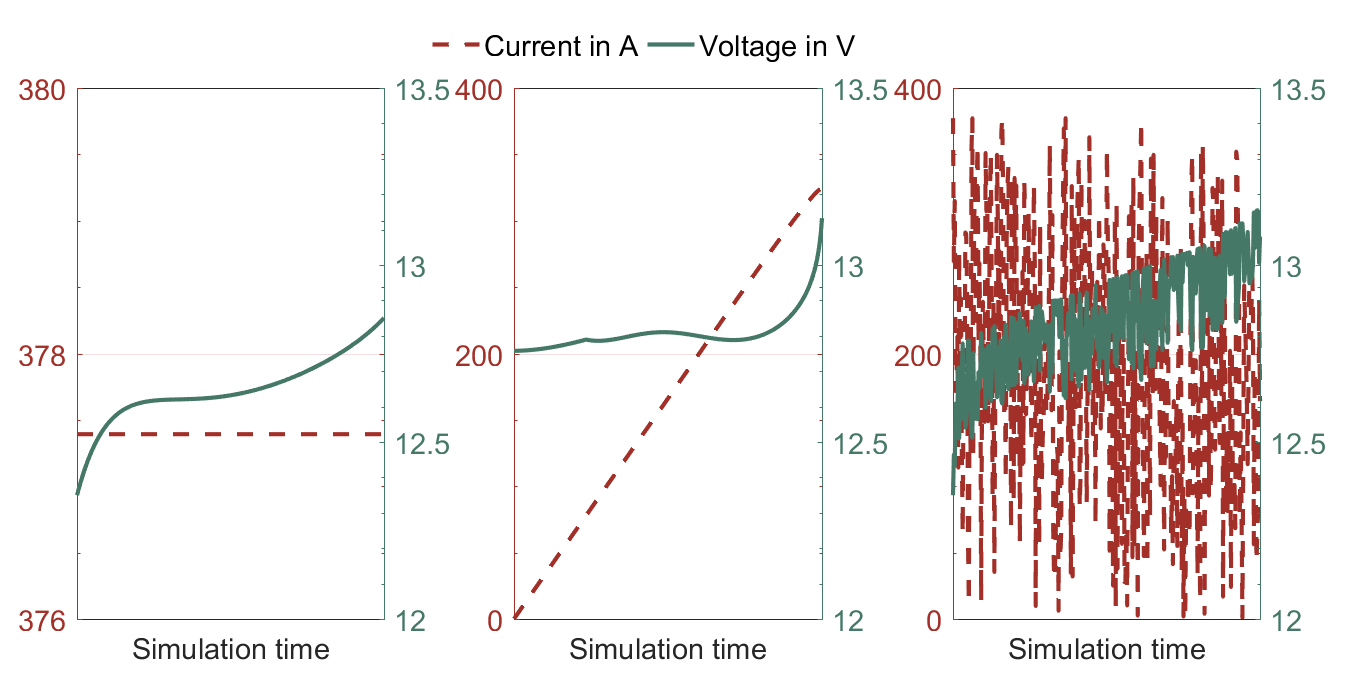
\includegraphics[width=\textwidth]{simulations01}
	\caption[Comparison of battery pack charging simulations using a constant current, a linearly increasing current and a random current, respectively - Voltage vs. simulation time]{Comparison of battery pack charging simulations using a constant current, a linearly increasing current and a random current, respectively - Voltage vs. simulation time. The pack's cells were modelled according to~\cite{_data_2010}.}
	\label{fig:simulations01}
\end{figure}
The results of three charging simulations of a battery pack are depicted in Figure~\ref{fig:simulations01}. Since the data sheet~\cite{_data_2010} that was used does not contain any voltage curves for charging currents, the discharge curves were used for charging, too\footnote{This is the default behaviour if no charge curves are added.}. Every time, the empty pack was charged until an $SoC$ of approx. 0.9 was reached. In the first simulation (on the left hand side), the battery was charged with a constant current $I\subi{max}$. The resulting voltage is an interpolation between two curve fits and appears to have perfect results upon first glance. For the second simulation (Figure~\ref{fig:simulations01}, centre), the current was linearly increased between 0 and $I\subi{max}$. The resulting voltage is a curve that interpolates all of the curve fits at different capacities.  Here, the problems of using discharge curves for charging become apparent. The voltage is higher than in the first simulation - especially at lower currents. This is typical behaviour for discharging. However, a lower charging current should result in lower voltages. Due to this problem, it is advisable to add separate charging and discharging curve fits to the model. This can be done via the \mcode{addcurves()} method:
\begin{lstlisting}
bat.addcurves(chargeCurvefitObj, 'charge')}
bat.addcurves(dischargeCurvefitObj, 'discharge')}
\end{lstlisting}
A charge curve fit can be fitted using the \mcode{dischargeFit} class or the \mcode{dischargeFit()} method (see section~\ref{sec:dischargeFit}) or a user-defined class that implements the \mcode{curveFitInterface}.
A random distribution of currents within the interval $[0, I\subi{max}]$ was used for the third simulation (Figure~\ref{fig:simulations01}, right). The main issue of this model's approach using curve fits is emphasised here. Voltage leaps occur if the current changes drastically from one time step to another. It is highly doubtful that a battery would behave like this in reality, since the discharge curves are actually measured by discharging with a certain current and then waiting for long periods of time (e.g. up to four hours) until the resting voltage stabilizes before taking measurements~\cite{keil_aufbau_2012}. A possible solution in a simulation that charges and discharges with strongly fluctuating currents could be to smooth the returned voltages out with a running mean or to use a customized version of the \mcode{dischargeCurves} class (see section~\ref{sec:dischargeCurves}) that always returns the mean of all currents' voltages as a function of the $SoC$. The \mcode{mdischargeCurves} class was added to this package for that purpose. As is shown in Figure~\ref{fig:simulations02}, plotting the voltage against the $SoC$ causes the curves to follow more similar functions than when plotting them against the current. By using the \mcode{mdischargeCurves} class instead of the \mcode{dischargeCurves} class, the volatile curve with random currents can be flattened out to produce the results in Figure~\ref{fig:mdischargeCurves}. It should be noted, however, that the mean charging and discharging currents of the simulation must be known so that the relevant curve fits can be added accordingly.
\begin{figure}[t!]
	\captionsetup{type=figure}
	\centering
	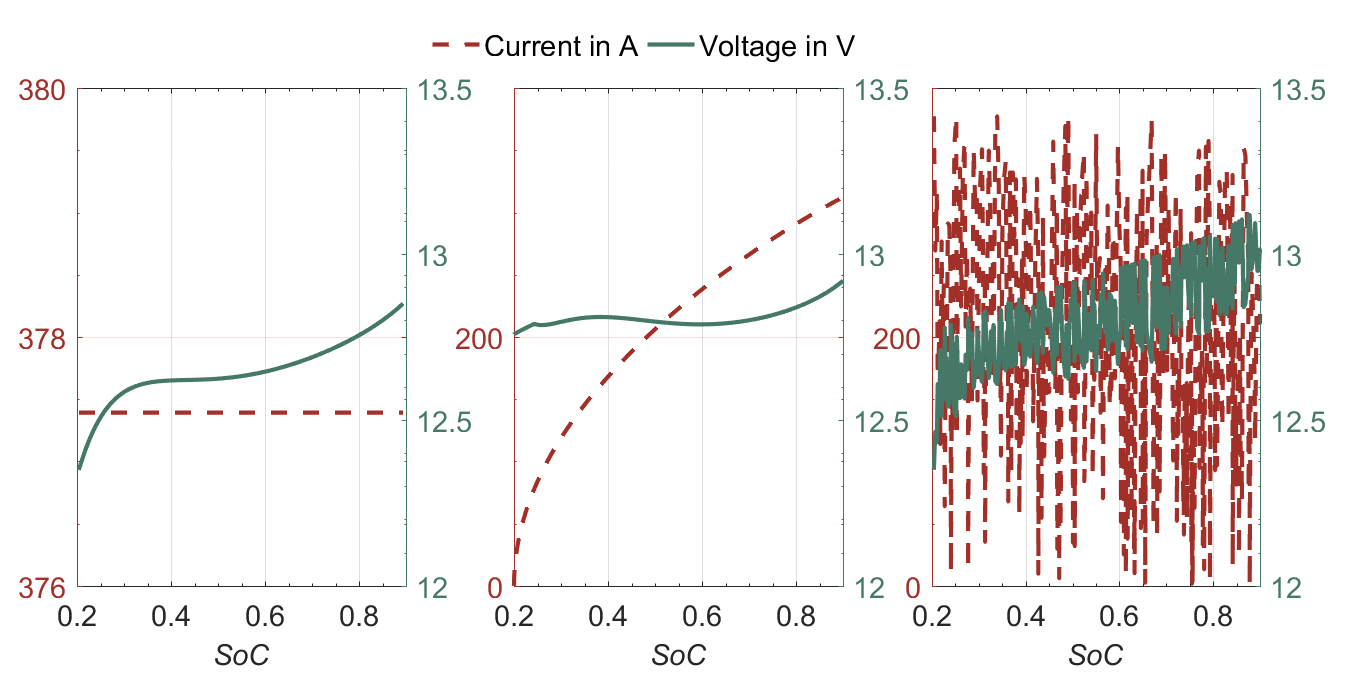
\includegraphics[width=\textwidth]{simulations02}
	\caption[Comparison of battery pack charging simulations using a constant current, a linearly increasing current and a random current, respectively - Voltage vs. $SoC$]{Comparison of battery pack charging simulations using a constant current, a linearly increasing current and a random current, respectively - Voltage vs. $SoC$. The pack's cells were modelled according to~\cite{_data_2010}.}
	\label{fig:simulations02}
\end{figure}
\begin{figure}[b!]
	\captionsetup{type=figure}
	\centering
	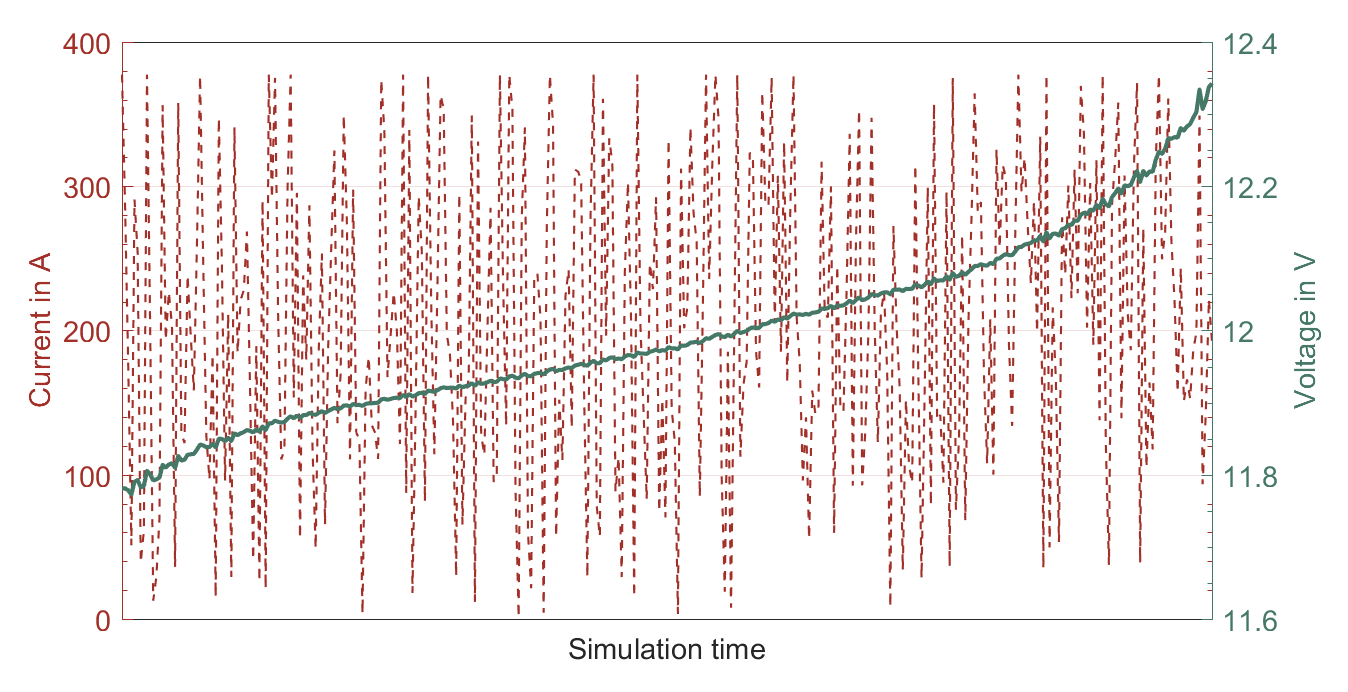
\includegraphics[width=\textwidth]{mdischargeCurves}
	\caption[Simulation of battery charging with random currents using the \mcode{mdischargeCurves} class for voltage calculation]{Simulation of battery charging with random currents using the \mcode{mdischargeCurves} class for voltage calculation. The resulting voltage is a function of the battery's $SoC$.}
	\label{fig:mdischargeCurves}
\end{figure}
\clearpage
An \mcode{mdischargeCurves} object shares the exact same interface as a \mcode{dischargeCurves} object. To convert the classes into each other, use the \mcode{add()} method.
\begin{lstlisting}
d2 = mdischargeCurves;
d2.add(d); % Adds all of the dischargeCurves' dischargeFit objects
		   % to the mdischargeCurves object
% Works the other way around, too
d = dischargeCurves;
d.add(d2)
\end{lstlisting}

\subsubsection{Age model level}
\label{sec:AgeModelLevel}
The age model (see section~\ref{sec:ageModel}) can be left out completely, added on the pack level or added on the cell level. Adding it on the pack level is done by calling \mcode{initAgeModel()}\footnote{The \mcode{initAgeModel()} method is described in sections~\ref{sec:cycleCounting}~-~\ref{sec:eoAgeModel}.} on the outermost wrapper object, e.g. a \mcode{batteryPack} (see section~\ref{sec:batteryPack}), a \mcode{parallelElement}, a \mcode{seriesElementPE}, etc. Doing so will cause the battery pack's total $SoC$ to be observed for cycle counting and the pack's $SoH$ to be updated by the \mcode{batteryAgeModel} object. If the cells have varying properties (i.e. different internal impedances), their individual cycles may vary and it could make sense to add an age model to each cell individually. This can be done by calling \mcode{initAgeModel()} on every cell. The cells can be extracted using the \mcode{createIterator()} method, which returns a \mcode{batteryIterator} object that can be used to iterate through the cells. To indicate that the age model is set to the cell, level, the main battery pack object (outermost wrapper) must have it's age model set to \mcode{'LowerLevel'}, or the $SoH$ will not be calculated correctly. The following code provides an example of extracting a battery pack \mcode{bat}'s cells and setting the age model.
\begin{lstlisting}
it = bat.createIterator;
while it.hasNext % Iterate through cells
	b = it.next; % batteryCell object
	b.initAgeModel('ageModel', 'EO')
end
% Make sure 'LowerLevel' option is set on outermost wrapper
bat.initAgeModel('LowerLevel')
\end{lstlisting}

\subsection{CCCV charging and BMS}
\label{sec:cccv_BMS}
\begin{figure}[t!]
	\captionsetup{type=figure}
	\centering
	\includegraphics[width=\textwidth]{cccv_qualitative}
	\caption[Qualitative example of a CCCV charging curve]{Qualitative example of a CCCV charging curve.}
	\label{fig:cccv_qualitative}
\end{figure}
Typically, a lithium-ion battery is charged using a constant current / constant voltage (CCCV) charging strategy. A qualitative example of the CCCV strategy is depicted in Figure~\ref{fig:cccv_qualitative}. In the CC phase, a constant charging current causes the $SoC$ to increase linearly over time while the voltage rises according to the respective charging curve (see section~\ref{sec:dischargeCurves}). When the voltage reaches a certain threshold, the current is reduced in order to stabilize the voltage during the CV phase. As a result, the $SoC$ is no longer a linear function of time and increases at a slower pace. In practice, this charging strategy works well for individual cells and cells connected in parallel, since the voltage is distributed evenly across all cells. However, this is not the case for cells connected in series. A CCCV charger may limit the total voltage, but it has no knowledge of the distribution across the individual cells, which could result in the cells with the highest voltage getting damaged~\cite{andrea_battery_2010}. To prevent this, a battery management system (BMS) is required. The BMS monitors each cell individually and communicates with the charger. In the case of active equalization, the BMS rebalances the charge and voltages among the cells. This can be modelled by using the \mcode{seriesElementAE} class (see section~\ref{sec:batteryCompositionOverview}).

\subsubsection{CCCV curve fits}
\label{sec:cccvFit}
Due to the fact that simulations using variable currents are possible with this model, the charge limitation in the CV phase is done by limiting the maximum charging current $I\subi{max}$ as a function of the $SoC$. Thus, lower currents than $I\subi{max}$ are also possible during the CC phase. By default, $I\subi{max}$ is limited according to the discharge curve with the largest current stored in the cell's \mcode{dischargeCurves} reference (see section~\ref{sec:charge_discharge}). If a set of charge curve fits is added without adding a CCCV curve (using the \mcode{'charge'} option of the \mcode{addcurves()} method), $I\subi{max}$ is set according to the charge curve with the greatest current. Finally, if a \mcode{cccvFit} object is added, $I\subi{max}$ is dynamically set as a linear function of the $SoC$ according to the CCCV curve fit. 
\begin{equation}
I\subi{max}(SoC) = \frac{I\subi{max,CC}}{1-SoC\subi{CC/CV}}\cdot (1 - SoC)
\end{equation}
where $I\subi{max,CC}$ is the maximum current during the CC phase and $SoC\subi{CC/CV}$ is the $SoC$ at the end of the CC phase.
To add a CCCV curve fit to a battery object \mcode{bat}, the \mcode{addcurvers()} method can be called with the \mcode{'cccv'} option. The \mcode{cccvFit} class implements the \mcode{curveFitInterface} and is initialized with the raw data ($SoC$ and $I\subi{max}$ with $I\subi{max} = f(SoC)$) and the optional name-value pairs described in section~\ref{sec:dischargeFit}. If for some reason the curve's maximum $SoC$ is not 1, it should be passed to the constructor via a third argument $SoC\subi{max}$.
\begin{lstlisting}
% CCCV curve fit
c = cccvFit(soc, iMax);
c2 = cccvFit(soc, iMax, socMax); % with SoC limitation
bat.addcurves(c, 'cccv') % add c to battery object
\end{lstlisting}
\begin{figure}[t!]
	\captionsetup{type=figure}
	\centering
	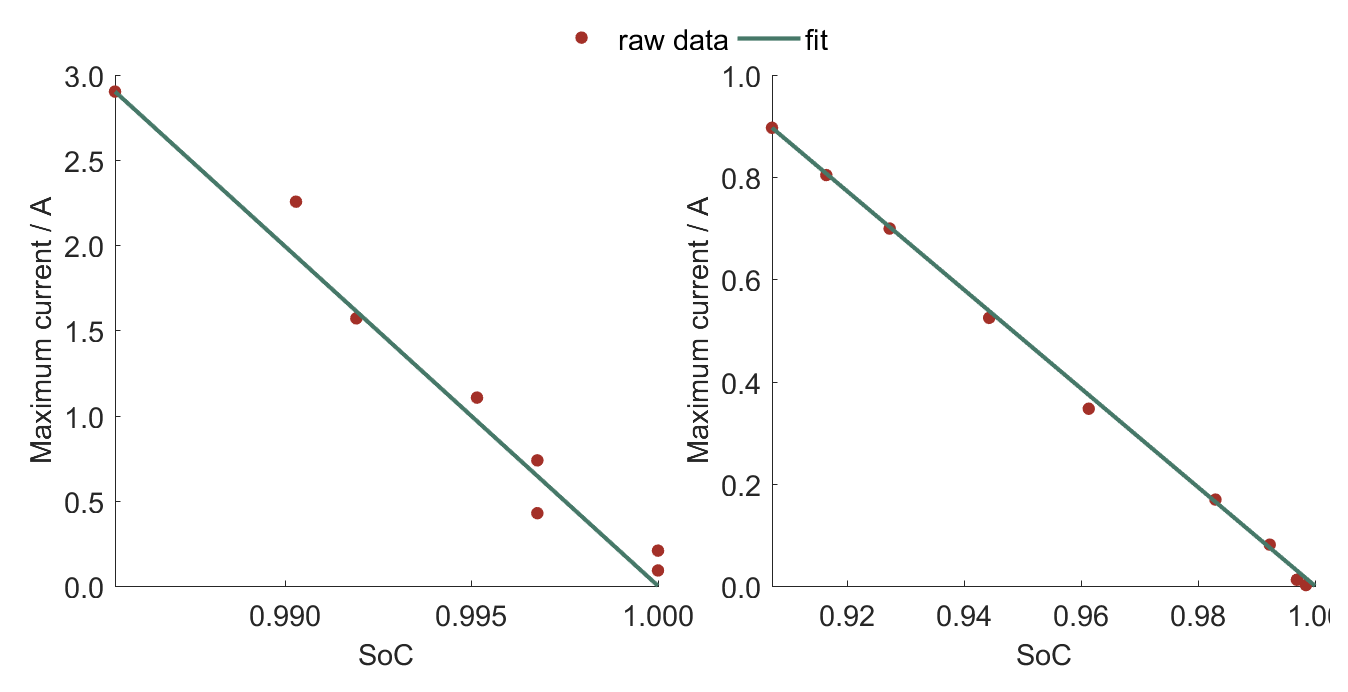
\includegraphics[width=\textwidth]{cccvFit}
	\caption[Linear curve fits of $I\subi{max}(SoC)$ during the CV phase for two different battery cells]{Linear curve fits of $I\subi{max}(SoC)$ during the CV phase for two different battery cells.}
	\label{fig:cccvFit}
\end{figure}
Two curve fits for two different battery cells' CV phases are depicted in Figure~\ref{fig:cccvFit}. For the cell fitted on the right hand side, the linear model provides a very good approximation. However, for cells with short CV phases resulting in small $SoC$ gradients (fitted on the left hand side), the digitized raw data can appear more noisy due to the difficulty in digitizing the image.

\subsubsection{Cell monitoring and communication with the charger}
\label{sec:BMS}
In this model, the cell monitoring and communication with the charger are implemented using the Observer design pattern. The cells take on the role of the subjects and are automatically registered with the pack they are added to via the \mcode{addElements()} method (see section~\ref{sec:batteryInterface}). The communication flows between the BMS and the charger are visualized in Figure~\ref{fig:cccvBMS}, with each communication path colour coded. Each battery composite object (e.g. a battery pack) contains a logical flag that indicates whether CV charging is active (true) or not (false). If a cell's individual $SoC$ reaches the threshold at which CV charging is activated, the battery pack is notified, causing it's flag to be set true. This notification is also sent out if a cell that was in the CV phase moves back into the CC phase by being discharged. At the beginning of each time step, the maximum charging current is recalculated if the battery pack's CCCV flag is true. This also sets it false again to prevent unnecessary recalculations. If the flag is false, charging continues with the last cached $I\subi{max}$. Using this method significantly reduces simulation time compared to directly triggering a recalculation of $I\subi{max}$ every time a cell's $SoC$ threshold is reached.  
\begin{figure}[t!]
	\captionsetup{type=figure}
	\centering
	\includegraphics[width=\textwidth]{cccvBMS}
	\caption[Schematic visualization of the BMS combined with CCCV charging]{Schematic visualization of the BMS combined with CCCV charging.}
	\label{fig:cccvBMS}
\end{figure}

\subsection{Simplified model}
The cell resolution of the battery model provided in this package can lead to long simulation times for packs containing large numbers of cells. For example, a 12~V pack with a capacity of 390~Ah (ca. 4.7~kWh) may contain over 500 cells (assuming a nominal cell voltage of 3.2~V and a nominal cell capacity of 3~Ah). In many simulations, the individual ageing and voltage distribution of cells may be of little to no interest. For such cases, a simplified version of the model was devised. It was implemented using the Decorator design pattern, which functions similarly to the Composite pattern used for the non-simplified model (see section~\ref{sec:batteryCompositionOverview}). The decorator (wrapper) objects used in the simplified model are
\begin{itemize}
	\item \mcode{simplePE}: A set of components in parallel.
	\item \mcode{simpleSE}: A set of components in series.
\end{itemize}
Much like the their non-simplified counterparts, they can hold a reference to either a \mcode{batteryCell} or another wrapper object. The difference is that the decorator can only wrap a single object, rather than an array of objects. The number of subcomponents is stored as a separate property. Instead of simulating individual cells and delegating the methods to each of the subcomponents (see section~\ref{sec:method_delegation}), the methods are delegated to a single subcomponent (and ultimately to a single cell) and the number of subcomponents is used to determine the end result. Consequentially, passive equalization cannot be modelled using the simplified model. Also, the age model can only be added on the pack level\footnote{It is technically possible to add an age model to the cell, but doing so has no effect other than slowing down the simulation if the \mcode{'LowerLevel'} argument is not passed to the pack's \mcode{initAgeModel()} method.}. While the \mcode{simplePE} and \mcode{simpleSE} classes do implement the \mcode{batteryInterface} and thus share all methods, their constructors are called differently. To construct a "simple circuit element" decorator, the wrapped object and the number of subcomponents it holds are passed as input arguments.
\begin{lstlisting}
b1 = batteryCell(3, 3.2);
b2 = batteryCell(3, 3.2);
% add dischargeCurves, etc. to b1 & b2...
se = simpleSE(b2, 3); % 3 cells in series
pe = simplePE(b1, 3); % 3 parallel cells
sp = simpleSE(pe, 3); % 3 strings of parallel elements
ps = simplePE(se, 3); % 3 parallel strings of cells
ps.initAgeModel('ageModel', 'EO') % initialize age model
\end{lstlisting}


\subsection{The \mcode{batteryPack} class}
\label{sec:batteryPack}
For simple, centralized access to most features of this package, a facade of the model was created in the form of the \mcode{batteryPack} class. In most use cases, the \mcode{batteryPack} will be the only class that needs to be accessed in order to create a fully functional battery pack model. The class contains methods for curve fitting and static functions that launch GUIs for digitizing the curves and easy configuration of the model (see section~\ref{sec:GUI}). Disregarding the \mcode{dischargeCurves}, it is possible to create a fully functional battery pack model using the \mcode{batteryPack} constructor alone\footnote{A \mcode{dischargeCurves} object must be created beforehand and passed to the constructor or added after the initialization of the pack using the \mcode{dischargeFit()} or \mcode{addcurves()} method.}. Possible topologies of a \mcode{batteryPack} are SP, PS, strings of cells and parallel cells (see section~\ref{sec:batteryCompositionOverview}). For more complicated topologies, the pack must be created using the non-simplified circuit element wrappers. 

\subsubsection{The \mcode{batteryPack} constructor}
\label{sec:batteryPackConstructor}
When initializing a \mcode{batteryPack} object, the cells and circuit elements (simplified or non-simplified) are initialized automatically according to the constructor's input arguments. An "empty" \mcode{batteryPack} object is constructed with the nominal cell capacity \mcode{Cc} in Ah, the nominal cell voltage \mcode{Vc} in V and one of the following:
\begin{enumerate}\renewcommand{\labelenumi}{\roman{enumi})}
	\item Automatic setup: The pack's nominal capacity \mcode{Cp} and voltage \mcode{Vp} in Ah and V, respectively. 
	\item Manual setup: The number of parallel cells \mcode{np} and the number of cells in series \mcode{ns}.
\end{enumerate}
\begin{lstlisting}
bat = batteryPack(Cp, Vp, Cc, Vc); % (i) Automatic setup
bat = batteryPack(np, ns, Cc, Vc); % (ii) Manual setup 
% (np & ns must be integers)
\end{lstlisting}
In option (i), the cells are automatically arranged in such a way that the pack's resulting nominal capacity and voltage come as close as possible to \mcode{Cp} and \mcode{Vp}, respectively. If the first two input arguments are integers, option (ii) is called and the pack's nominals are calculated according to \mcode{np} and \mcode{ns}. To call option (ii) with any numeric data type, the \mcode{'Setup'} option must be set to \mcode{'Manual'}.
\begin{lstlisting}
bat = batteryPack(np, ns, Cc, Vc, 'Setup', 'Manual');
\end{lstlisting}
All of the above constructors can be called with additional options that are specified by the name-value pairs listed in Table~\ref{tab:batteryPackOptions}.
\begin{lstlisting}
bat = batteryPack(.., 'OptionName', OptionValue);
\end{lstlisting}
If no \mcode{dischargeCurves} object is passed to the \mcode{batteryPack} via it's constructor's \mcode{'dCurves'} option, a warning is printed to the command window. A warning is also printed if an age model is specified (using the \mcode{'ageModel'} option), but no cycle life curve fit (i.e. \mcode{woehlerFit}) object is passed via the \mcode{'ageCurve'} option. The model cannot be used until a \mcode{dischargeCurve} is initialized (either via the constructor or via the \mcode{dischargeFit()} or \mcode{addcurves()} method).

\begin{longtable}{l l m{0.45\textwidth}l}
	\caption[Option name-value pairs of the \mcode{batteryPack} constructor]{Option name-value pairs of the \mcode{batteryPack} constructor.}\\ \toprule
	Name & Values & Description \\ \midrule
	\endfirsthead
	\multicolumn{3}{@{}l}{\ldots continued}\\
	\toprule
	Name & Values & Description \\ \midrule
	\endhead
	\hline
	\multicolumn{3}{r@{}}{continued \ldots}\    \endfoot
	\bottomrule
	\endlastfoot
	\mcode{'ageCurve'} & \tml{\mcode{'none'} (default)\\ Age curve object} & Adds an age curve (e.g. \mcode{woehlerFit}) to the battery's age model.\\
	\midrule
	\mcode{'ageModel'} & \tml{\mcode{'none'} (default) \\ \mcode{'EO'} \\ Age model object}& 
	Specifies the age model that is used. \mcode{'EO'} stands for "event oriented aging". Optionally, a custom age model object that implements the \mcode{batteryAgeModel} interface can be passed as a value.\\
	\midrule
	\mcode{'AgeModelLevel'} & \tml{\mcode{'Pack'} (default) \\ \mcode{'Cell'}} & Specifies whether the age model is applied to the pack or to each cell individually.\\
	\midrule
	\mcode{'cccvCurves'} & \tml{\mcode{'none'} (default)\\ CCCV curve fit} & Adds a CCCV curve fit object (e.g. \mcode{cccvFit}) to the battery's cells for charge current limitation in the CV phase.\\
	\midrule
	\mcode{'cCurves'} & \tml{\mcode{'none'} (default)\\ Charge curve fit} & Adds a Charge curve fit object (e.g. \mcode{curvefitCollection} subclass) to the battery's cells for voltage calculation during charging.\\
	\midrule
	\mcode{'cycleCounter'} & \tml{\mcode{'auto'} (default) \\ \mcode{'dambrowski'} \\ Cycle counter object} & Specifies the class that is used for cycle counting. By default, no counter is selected if no age model is specified. Otherwise, a \mcode{dambrowskiCounter} is used. A custom cycle counter object that implements the \mcode{cycleCounter} interface can also be passed as a value.\\
	\midrule
	\mcode{'dCurves'} & \tml{\mcode{'none'} (default)\\ Discharge curve fit} & Adds a discharge curve fit object (e.g. \mcode{dischargeCurves}) to the battery's cells.\\
	\midrule
	\mcode{'Equalization'} & \tml{\mcode{'Passive'} (default) \\ \mcode{'Active'}} & Specifies which type of equalization (balancing) is used for the strings in the pack. If the \mcode{'ideal'} option is set to true, active equalization is is always used.\\
	\midrule
	\mcode{'etaBC'} & \tml{\mcode{1x1 double} \\ Default: $0.97$} & The battery's charging efficiency. Must be between $0$ and $1$.
	If the data sheet does not differentiate between charging and discharging efficiencies, set this property according to the data sheet and \mcode{'etaBD'} to $1$.\\
	\midrule
	\mcode{'etaBD'} & \tml{\mcode{1x1 double} \\ Default: $0.97$} & The battery's discharging efficiency. Must be between $0$ and $1$.\\
%	\midrule
	\mcode{'ideal'} & \tml{\mcode{false} (default) \\ \mcode{true}} & If set to true, the battery is constructed using the faster, simplified model with ideal cells and balancing. Setting this to true assumes that all cells have exactly the same parameters and that the balancing is perfect. This should result in much fewer resource consumption during simulation, as only one cell is used for calculations.\\
	\midrule
	\mcode{'psd'} & \tml{\mcode{1x1 double}\\ Default: $0$} & Self-discharge in $1$/month. Must be between $0$ and $1$ (i.e. $0.01$ for a self-discharge of $1$~\% per month)\\
	\midrule
	\mcode{'socMax'} & \tml{\mcode{1x1 double}\\ Default: $1$} & Upper limit for the battery pack's $SoC$.\\
	\midrule
	\mcode{'socMin'} & \tml{\mcode{1x1 double}\\ Default: $0.2$} & Lower limit for the battery pack's $SoC$. Note that the $SoC$ can go below this limit if it is above $0$ and if the self-discharge (\mcode{'psd'}) has been set to a value greater than $0$.\\
	\midrule
	\mcode{'socIni'} & \tml{\mcode{1x1 double}\\ Default: $0.2$} & Initial $SoC$ of the battery pack.\\
	\midrule
	\mcode{'sohIni'} & \tml{\mcode{1x1 double}\\ Default: $1$} & Initial $SoH$ of the battery pack.\\
	\midrule
	\mcode{'Topology'} & \tml{\mcode{'SP'} (default)\\ \mcode{'PS'}} & The topology of the pack's cells. \mcode{'SP'} for strings of parallel cells and \mcode{'PS'} for parallel strings of cells\\
	\midrule
	\mcode{'Zi'} & \tml{\mcode{1x1 double}\\ Default: $17\cdot 10^{-3}$} & Internal impedance of the battery cells in $\Omega$. The internal impedance is currently not used as a physical parameter. However, it is used in the circuit elements to determine the distribution of currents and voltages.\\
	\midrule
	\mcode{'Zgauss'} & \tml{\mcode{1x3 double}\\ Default \mcode{[0, Zi, Zi]}} & Vector for gaussian distribution of the battery cells' internal impedances. The vector has the following values: \mcode{[Zstd, Zmin, Zmax]} with \mcode{Zstd}~=~Standard deviation std of the internal impedance $Z\subi{i}$ in $\Omega$; \mcode{Zmin}~=~Smallest $Z\subi{i}$ in $\Omega$ and \mcode{Zmax}~=~Largest $Z\subi{i}$ in $\Omega$. The mean is the value specified by the option \mcode{'Zi'}. This setting is ignored if the \mcode{'ideal'} option is set to \mcode{true}. In order to use this option, the Statistics and Machine Learning Toolbox must be installed. Due to the limitation of $Z\subi{i}$ to \mcode{Zmin} and \mcode{Zmax}, the mean or std may vary slightly from what was set. To get an exact std, \mcode{Zmin} must be set to \mcode{-Inf} and \mcode{Zmax} must be set to \mcode{Inf}\footnote{A Gaussian distribution is mathematically defined for the interval $[-\infty, \infty]$. In this package, the interval can be limited iteratively using the \mcode{norminvlim()} function~\cite{jakobi_norminvlim_2016}, but a perfect limitation is not possible.}.
	\label{tab:batteryPackOptions}
\end{longtable}

\subsubsection{Properties of the \mcode{batteryPack} class}
The accessible properties of the \mcode{batteryPack} class are listed in Table~\ref{tab:batteryPackProps}. With the exception of \mcode{AgeModelLevel}, all properties are inherited from the \mcode{batteryInterface} and are therefore also available for all other \mcode{batteryInterface} subclasses, such as the \mcode{batteryCell}, \mcode{parallelElement}, etc.
\begin{longtable}{l p{0.47\textwidth}l l l}
	\caption[Accessible properties of the \mcode{batteryPack} class]{Accessible properties of the \mcode{batteryPack} class.}\\ \toprule
	Property & Description & Unit & Set access \\ \midrule
	\endfirsthead
	\multicolumn{3}{@{}l}{\ldots continued}\\
	\toprule
 	Property & Description & Unit & Set access \\ \midrule
	\endhead
	\hline
	\multicolumn{3}{r@{}}{continued \ldots}\    \endfoot
	\bottomrule
	\endlastfoot
	\mcode{AgeModelLevel} & Level of the age model (\mcode{'Cell'} or \mcode{'Pack'}) & - & read only \\
	\mcode{C} & Current capacity level & Ah & read only \\
	\mcode{Cbu} & Total useable capacity taking $SoH$ and $SoC$ boundaries into account & Ah & read only \\
	\mcode{Cd} & Discharge capacity & Ah & read only \\
	\mcode{Cn} & Nominal (or average) capacity & Ah & immutable \\
	\mcode{eta_bc} & Efficiency when charging & - & immutable \\
	\mcode{eta_bd} & Efficiency when discharging & - & immutable \\
	\mcode{ImaxC} & Maximum charging current & A & read only \\
	\mcode{ImaxD} & Maximum discharging current & A & read only \\
	\mcode{psd} & Self discharge rate & $1$/month & immutable \\
	\mcode{SoC} & State of charge & - & read only \\
	\mcode{socMax} & Maximum $SoC$ & - & public \\
	\mcode{socMin} & Minimum $SoC$ & - & public \\
	\mcode{SoH} & State of health & - & read only \\
	\mcode{V} & Resting voltage & V & read only \\
	\mcode{Vn} & Nominal (or average) voltage & V & read only \\
	\mcode{Zi} & Internal impedance & $\Omega$ & immutable \\
	\mcode{nP} & number of parallel elements & - & read only \\
	\mcode{nS} & number of elements in series & - & read only \\
	\mcode{maxIterations} & Maximum number of iterations in the \mcode{iteratePower()} and \mcode{iterateCurrent()} methods & - & public \\
	\mcode{pTol} & Tolerance for the power iteration (Stopping criteria) & W & public \\
	\mcode{sTol} & Tolerance for the $SoC$ limitation iteration & - & public \\
	\label{tab:batteryPackProps}
\end{longtable}

\subsubsection{Methods of the \mcode{batteryPack} class}
As a subclass of the \mcode{batteryInterface}, all of it's methods are inherited by the \mcode{batteryPack} class. For a detailed description of battery charging and discharging using the \mcode{powerRequest()} and/or \mcode{currentRequest()} methods, see section~\ref{sec:charge_discharge}. These are the two methods that are required for the simulation. Most of the class's public methods are only needed for internal algorithms of the model. However, a complete list of the public methods is provided in Table~\ref{tab:batteryPackMethods}. The curve fitting methods (which can be called if curve fits are not passed to the constructor) and the GUI tool functions are not inherited from the \mcode{batteryInterface}. A detailed description of the syntax of each method with the respective input and output arguments is provided in the \matlab\ documentation, which can be accessed by typing
\begin{lstlisting}
doc lfpBattery.batteryPack % or
import lfpBattery.*
doc batteryPack
\end{lstlisting}
into the command window.

\begin{longtable}{l p{0.6\textwidth}l}
	\caption[Public methods of the \mcode{batteryPack} class]{Public methods of the \mcode{batteryPack} class.}\\ \toprule
	Method & Description\\ \midrule
	\endfirsthead
	\multicolumn{3}{@{}l}{\ldots continued}\\
	\toprule
	Method & Description\\ \midrule
	\endhead
	\hline
	\multicolumn{3}{r@{}}{continued \ldots}\    \endfoot
	\bottomrule
	\endlastfoot
	\mcode{powerRequest()} & Requests a power in W (positive for charging,
	negative for discharging) from the battery. \\
	\mcode{iteratePower()} & Iteration to determine new state given a certain power. The state of the battery is not changed by this method. \\
	\mcode{currentRequest()} & Requests a current in A (positive for charging,
	negative for discharging) from the battery.  \\
	\mcode{iterateCurrent()} & Iteration to determine new state given a certain current. The state of the battery is not changed by this method. \\
	\mcode{addCounter()} & Registers a cycleCounter object as an observer\footnote{Not recommended. Use \mcode{initAgeModel()} instead.}. \\
	\mcode{dischargeFit()}\footnote{Unique to the \mcode{batteryPack} class.} & Uses Levenberg-Marquardt algorithm to fit a
	discharge curve. \\
	\mcode{chargeFit()}\footnotemark[2]. & Uses Levenberg-Marquardt algorithm to
	fit a charge curve. \\
	\mcode{cycleFit()}\footnotemark[2] & Creates a fit object for a cycles to
	failure vs. DoD curve and adds it to the pack. \\
	\mcode{cccvFit()}\footnotemark[2] & Adds a CCCV curve fit to the pack. \\
	\mcode{initAgeModel()} & Initializes the age model of the battery. \\
	\mcode{getNewDischargeVoltage()} & Returns the new voltage according to a discharging current and a time step size. The state of the battery is not changed by this method. \\
	\mcode{getNewChargeVoltage()} & Returns the new voltage according to a charging current and a time step size. \\
	\mcode{addcurves()} & Adds a collection of discharge/charge curves, a cycle
	life curve or a CCCV curve to the battery. \\
	\mcode{randomizeDC()}\footnotemark[2] & Slight randomization of each cell's discharge
	curve fits\footnote{Not recommended. This method is an alternative to setting a gaussian distribution of the internal impedances $Z\subi{i}$. However, this method may use large amounts of memory and result in degraded performance.}. \\
	\mcode{digitizeTool()}\footnotemark[2] & (Static) Opens a GUI for digitizing discharge curves and cycle life curves (requires JAVA). \\
	\mcode{GUI}\footnotemark[2] & (Static) Opens a GUI for creating a batteryPack model (requires JAVA). \\
	\label{tab:batteryPackMethods}
\end{longtable}